
\section{Time Dilation from Relative Motion}

First, consider time dilation for a particle moving at high speed relative to the æther rest frame. Empirically, we know that a clock moving at velocity $v$ experiences time slower by the Lorentz factor $\gamma = 1/\sqrt{1 - v^2/c^2}$. In this model, we derive the same effect by analyzing the influence of absolute æther motion on vortex core rotation.

\subsection*{(a) Kinematic Derivation}

Let a vortex be at rest in its own frame $S'$ but moving at velocity $v$ relative to the æther rest frame $S$. In $S'$, the vortex rotates with angular frequency $\omega_0$, and defines proper time $\tau$. Due to Lorentz time dilation, an observer in $S$ sees the clock slow down:

\begin{figure}[htbp]
    \centering
    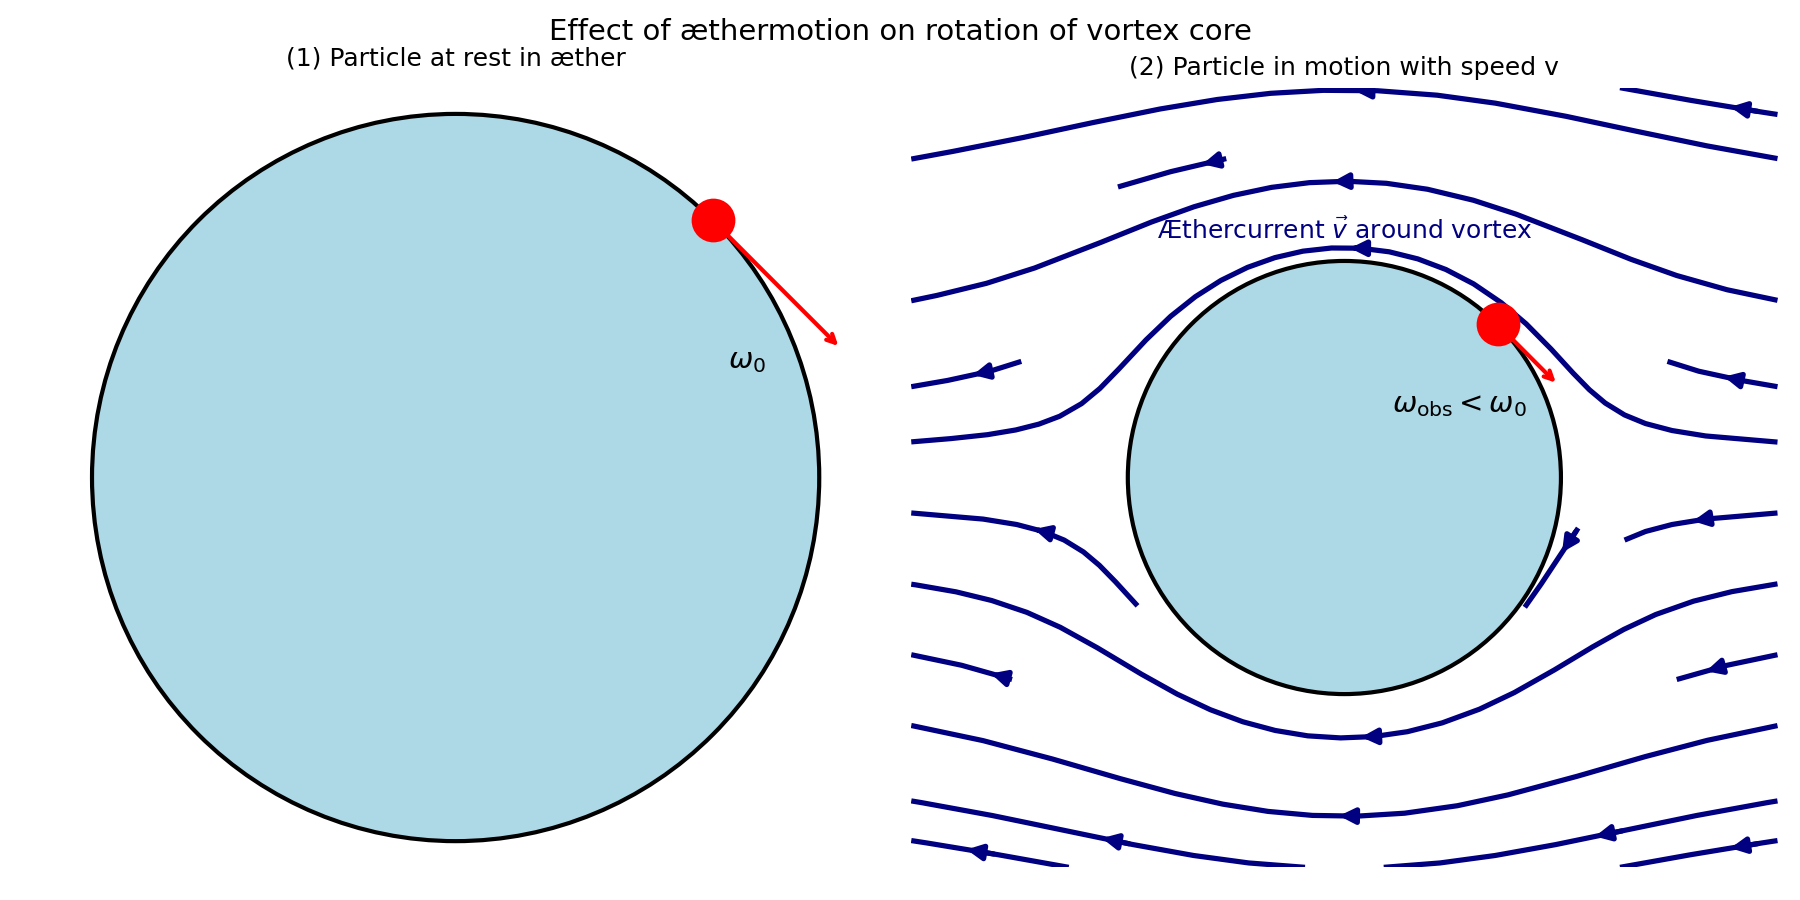
\includegraphics[width=0.85\textwidth]{06-TijdsdilatatieBeweging}
    \caption{Effect of æther flow on the internal rotation velocity of a vortex particle. At rest (left), the vortex retains its maximum angular velocity~$\omega_0$. When moving through the æther (right), the flow causes a reduced observed angular velocity to~$\omega_{\mathrm{obs}} < \omega_0$.}
    \label{fig:TijdsdilatatieBeweging}
\end{figure}

\[
\omega_{\text{obs}} = \omega_0 \sqrt{1 - \frac{v^2}{c^2}} \,.
\]
From the relation between proper and coordinate time,
\[
\frac{d\tau}{dt} = \frac{\omega_{\text{obs}}}{\omega_0} = \sqrt{1 - \frac{v^2}{c^2}} \,. \tag{2}
\]

This matches the standard SR time dilation formula. In our model, the physical mechanism is that æther motion across the vortex disrupts its swirl rate, slowing the apparent rotation in the æther frame.

\subsection*{(b) Fluid-Dynamic Interpretation}

A complementary interpretation uses compressible flow analogies. In fluid dynamics, a body moving at speed $v$ in a compressible medium with signal speed $c$ experiences distortions proportional to $\gamma = 1/\sqrt{1 - v^2/c^2}$. This can be thought of as a Doppler time dilation or resistance to maintaining coherent circulation. 

As velocity approaches the æther signal speed $c$, the surrounding flow compresses and resists vortex rotation. Therefore, the angular velocity seen in the æther frame drops, and:
\[
\omega_{\text{obs}} = \omega_0 \sqrt{1 - \frac{v^2}{c^2}} \Rightarrow \frac{d\tau}{dt} = \sqrt{1 - \frac{v^2}{c^2}} \,. \tag{3}
\]


In fluid dynamics, the Prandtl–Glauert factor explicitly characterizes compressible flow disturbances around objects moving near a medium’s characteristic signal speed $c$. As velocity approaches this speed, fluid disturbances become increasingly resistant to propagation forward, closely analogous to the ætheric reduction of vortex core rotation at high velocities. Thus, the emergence of the Lorentz factor $\gamma$ in our model is physically and mathematically analogous to fluid compressibility effects.


\subsection*{Implication}

This gives us the relativistic time dilation for a moving clock:
\[
\boxed{\frac{d\tau}{dt} = \sqrt{1 - \frac{v^2}{c^2}}}
\]
within a Euclidean, æther-based flat space, and matches all special relativity experimental predictions~\cite{Rado2020-aether-Lorentz,Levy2009-aether-clock}.